\documentclass{standalone}
\usepackage{tikz}
\usepackage{ctex,siunitx}
\usepackage{tkz-euclide}
\usepackage{amsmath}
\usetikzlibrary{patterns, calc}
\usetikzlibrary {decorations.pathmorphing, decorations.pathreplacing, decorations.shapes,}
\begin{document}
\small
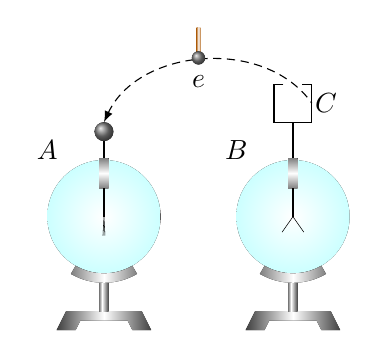
\begin{tikzpicture}[>=latex,scale=1.2]
  % \useasboundingbox(-1,-2)rectangle(8,6);
  \fill[inner color=white, outer color=cyan!20](0,0)circle(0.6);
  \fill[left color=darkgray,right color=darkgray, middle color=white](-0.5,-1.2)--++(0.2,0)--++(0.05,0.1)--++(0.5,0)--++(0.05,-0.1)--++(0.2,0)--++(-0.1,0.2)--++(-0.8,0)--cycle;
  \fill[left color=gray,right color=white](-0.05,-0.6)rectangle(-0.02,-1.0);
  \fill[left color=white,right color=darkgray](-0.02,-0.6)rectangle(0.05,-1.0);
  \fill[left color=gray,right color=gray, middle color=white](300:0.6)arc(300:240:0.6)--(240:0.7)arc(240:300:0.7)--cycle;
  \fill[top color=gray,bottom color=gray,middle color=white](-0.05,0.3)rectangle(0.05,0.62);
  \draw(0,0.62)--(0,1.0);
  \draw(0,0.3)--(0,0);
  \draw[very thin](0,0)--(267:0.2)(0,0)--(273:0.2);
  \fill[ball color=gray](0,0.9)circle(0.1);
  \node at (-0.6,0.7) {$A$};
  \begin{scope}[xshift=2cm]
    \fill[inner color=white, outer color=cyan!20](0,0)circle(0.6);
  \fill[left color=darkgray,right color=darkgray, middle color=white](-0.5,-1.2)--++(0.2,0)--++(0.05,0.1)--++(0.5,0)--++(0.05,-0.1)--++(0.2,0)--++(-0.1,0.2)--++(-0.8,0)--cycle;
  \fill[left color=gray,right color=white](-0.05,-0.6)rectangle(-0.02,-1.0);
  \fill[left color=white,right color=darkgray](-0.02,-0.6)rectangle(0.05,-1.0);
  \fill[left color=gray,right color=gray, middle color=white](300:0.6)arc(300:240:0.6)--(240:0.7)arc(240:300:0.7)--cycle;
  \fill[top color=gray,bottom color=gray,middle color=white](-0.05,0.3)rectangle(0.05,0.62);
  \draw(0,0.62)--(0,1.0)(-0.1,1.4)--(-0.2,1.4)--(-0.2,1.0)--(0.2,1.0)--(0.2,1.4)--(0.1,1.4);
  \draw(0,0.3)--(0,0);
  \draw[very thin](0,0)--(235:0.2)(0,0)--(305:0.2);
  \node at (-0.6,0.7) {$B$};
  \node at (0.35,1.2) {$C$};
  \end{scope}
  \draw[densely dashed,<-] (0,1.0) to[bend left=60] (2.2,1.2);
  \fill[left color=brown,right color=brown,middle color=white](0.98,1.7)rectangle(1.02,2.0);
  \fill[ball color=gray](1.0,1.68)circle(0.07)node[below=1mm]{$e$};
\end{tikzpicture}
\end{document}